\documentclass[a4paper, 12pt]{article} % тип документа

%%%Библиотеки
	%\usepackage[warn]{mathtext}	
	\usepackage[T2A]{fontenc}   %Кодировка
	\usepackage[utf8]{inputenc} %Кодировка исходного текста
	\usepackage[english, russian]{babel} %Локализация и переносы
	\usepackage{caption}
	\usepackage{listings}
	\usepackage{amsmath, amsfonts, amssymb, amsthm, mathtools}
	\usepackage[warn]{mathtext}
	\usepackage[mathscr]{eucal}
	\usepackage{wasysym}
	\usepackage{graphicx} %Вставка картинок правильная
	\DeclareGraphicsExtensions{.pdf,.png,.jpg}
	\graphicspath{ {images/} }
	
	\setlength{\parskip}{0.5cm}
	
	\usepackage{pgfplots}
	\usepackage{indentfirst}
	\usepackage{float}    %Плавающие картинки
	\usepackage{wrapfig}  %Обтекание фигур (таблиц, картинок и прочего)
	\usepackage{fancyhdr} %Загрузим пакет
	\usepackage{lscape}
	\usepackage{xcolor}
	\usepackage[normalem]{ulem}
	\usepackage{wasysym}
	\usepackage{subfig}
	\usepackage{graphicx}
	
	\usepackage{titlesec}
	\titlelabel{\thetitle.\quad}

	\usepackage{hyperref}
	\newenvironment{comment}{}{}

%%%Конец библиотек

%%%Настройка ссылок
%%%	\hypersetup
%%%	{
%%%		colorlinks = true,
%%%		linkcolor  = blue,
%%%		filecolor  = magenta,
%%%		urlcolor   = blue
%%%	}
%%%Конец настройки ссылок


%%%Настройка колонтитулы
    \pagestyle{fancy}
    \fancyhead{}
    \fancyhead[L]{1.1.1}
    \fancyhead[R]{Засимов Георгий, группа Б01-109}
    \fancyfoot[C]{\thepage}
%%%конец настройки колонтитулы


\usepackage[T2A]{fontenc}			% кодировка
\usepackage[utf8]{inputenc}			% кодировка исходного текста
\usepackage[english,russian]{babel}	% локализация и переносы
\usepackage{tikz}
\usepackage{pgfplots}


% Математика
\usepackage{amsmath,amsfonts,amssymb,amsthm,mathtools} 


\usepackage{wasysym}

\begin{document}

%%%Начало титульника
\begin{titlepage}

    \newpage
    \begin{center}
        \normalsize Московский физико-технический институт \\(национальный исследовательский университет)
    \end{center}

    \vspace{6em}

    \begin{center}
        \Large Лабораторная работа по общему курсу физики\\
    \end{center}

    \vspace{1em}

    \begin{center}
        \Large \textbf{Отчёт о выполнении лабораторной работы 1.4.8\\ {Измерение модуля Юнга методом акустического резонанса.}}
    \end{center}

    \vspace{2em}

    \begin{center}
        \large Засимов Георгий Алексеевич \\
        Группа Б01-109
    \end{center}

    \vspace{\fill}

    \begin{center}
    Долгопрудный \\2021
    \end{center}
    
\end{titlepage}
%%%Конец Титульника

\newpage

%\\\\\\\\\\\\\\\\\\\\\\\\\\\\\\\\\\\\\\\\\\\\\\\\\\\\\\\\\\\\\\\\\\\\\\\\\\\\
\section{Аннотация}

    В данной работе по результатам измереиний строится график зависимости частоты гармонических колебаний от номера гармоники для каждого из трёх металлических стержней (из меди, стали и алюминия), проверяется, что эта зависимость линейна. Рассчитывается значение скорости звука по полученным экспериментальным точкам. Определяется модуль Юнга для каждого из металлов - меди, алюминия и стали.


\section{Теоретические сведения и методика измерений}

    Модуль Юнга - оснавная характеристика упругих свойств твердого тела. По закону Гука при приложении к телу некоторого кратковременного напряжения $\sigma$ в теле возникает малая деформация, которая распространяется по телу вдоль оси приложения напряжения в форме акустической (звуковой) волны. Скорость этой волны $u$ можно найти по формуле ($\rho$ - плотность тела, Е - модуль Юнга тела):
\begin{equation} \label{скорость звука}
    u = \sqrt{\frac{E}{\rho}}
\end{equation}


    В данной работе мы рассматриваем длинные тонкие стержни. Звукавая волна в таком стержне распространяется только вдоль его длины и он испытывает деформации по закону Гука, а следовательно его упругие свойства описываются только модулем Юнга.При необходимой длине акустической волны в длине стержня помещается целое количество полуволн и при отражении волн от краев стержня происходит акустический резонанс.
    
    
    Волновое уравнение имеет вид ($u$ - скорость распространения волны, $\xi (x, t)$ - относительное удлинение элемента стержня в точке х к моменту $t$):
\begin{equation} \label{волновое уравнение}
    \frac{\delta^2\xi}{\delta t^2} = u^2 \frac{\delta^2\xi}{\delta x^2}
\end{equation}

    Решением данного уравнения является $\xi = \phi(x-ut)$ - произвольная функция, зависящая от $X = x - ut$. 
    
    Данная функция описывает возмущение среды произвольной формы, которое смещается поступательно во времени по оси х со скоростью $u$, не меняя своей формы. 
    
    При распространении волны против направления оси х решение волнового уравнения примет вид: $\xi =\phi(x+ut)$.
    
    Общее решение волнового уравнения имеет вид: $\xi =\phi_1(x-ut) + \phi_2(x+ut)$ - это сумма двух волн произвольной формы, бегущих в противоположные стороны со скоростями $\pm u$ (вид функций $\phi_1,\phi_2$ определяется из начальных и граничных условий задачи).
    
    
    
    
    Продольная волна в тонком стержне можетбыть представлена как суперпозиция бегущих навстречу гармонических волн:
    
\begin{equation}
    \xi (x, t) = A_1 Sin(\omega t - kx + \varphi_1) + A_2 Sin(\omega t + kx + \varphi_2)
\end{equation}

    где $\omega = 2\pi f$ - циклическая частота, $k = \frac{1\pi}{\lambda}$ - волновое число (пространственная частота) волны. Соотношения между амплитудами $A_1, A_2$ и начальными фазами $\varphi_1, \varphi_2$ определяются граничными условиями на концах стержня.
    
    
    
    Гармонические стоячие волны - это колебания вида ($A_1 = A_2, \varphi_1 = \varphi_2$):
    
\begin{equation}
    \xi (x, t) = 2A Cos(kx)Sin(\omega t + \varphi)
\end{equation}

    Из данного уравнения получаем, что на длине стержня должно укладываться целое число полуволн ($n \in N$):

\[\lambda_n = \frac{2L}{n}\]\\



    Собственные частоты колебаний стержня - допустимые значения 

\[f_n = \frac{u}{\lambda_n} = n\frac{n}{2L}\]

    Амплитуда колебаний смещения среды распределена вдоль стержня по гармоническому закону:
    
\begin{equation}
    \xi_0(x) = 2A Coskx
\end{equation}
    
    
    
    Точки с максимальной амплитудой (а значит и плотностью) - пучности смещения, с минимальной (нулевой) - узлы смещения.

    Номер гармоники $n$ определяет количество узлов смещения на стержне.
    
    
    
    
    
\section{Оборудование и экспериментальные погрешности}
\subsection{Экспериментальная установка}


\begin{center}
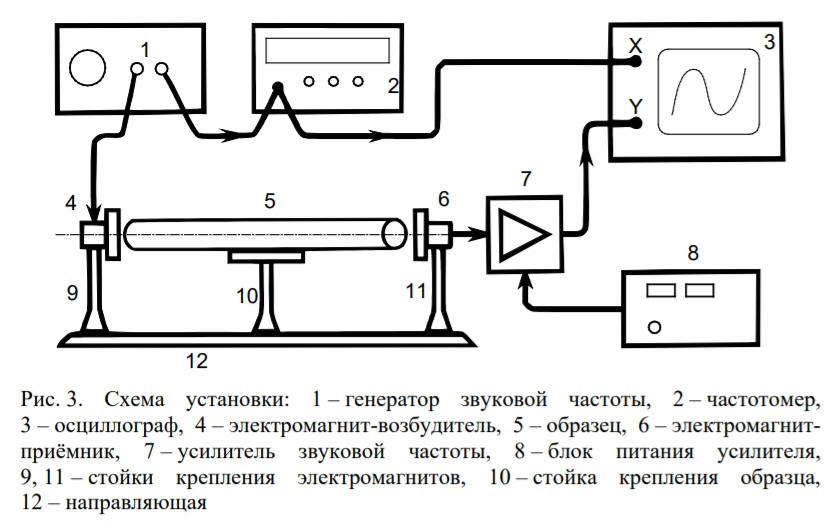
\includegraphics[width=15cm, height=11cm]{ustanovka.jpeg}
\end{center}


\begin{flushright}
{\scriptsize \textbf{Рис. 1} \textbf {Экспериментальная установка.}}
\end{flushright}



    Схема экспериментальной установки приведена на рис. 1. Исследуемый стержень 5 размещается на стойке 10. Возбуждение и приём колебаний в стержне осуществляются электромагнитными преобразователями 4 и 6, расположенными рядом с торцами стержня. Крепления 9, 11 электромагнитов дают возможность регулировать их расположение по высоте, а также перемещать вправо-влево по столу 12. Электромагнит 4 служит для возбуждения упругих механических продольных колебаний в стержне. На него с генератора звуковой частоты 1 подаётся сигнал синусоидальной формы: протекающий в катушке электромагнита ток создаёт пропорциональное ему магнитное поле, вызывающее периодическое воздействие заданной частоты на торец стержня (к торцам стержней из немагнитных материалов прикреплены тонкие стальные шайбы). Рядом с другим торцом стержня находится аналогичный электромагнитный датчик 6, который служит для преобразования механических колебаний в электрические. Сигнал с выхода генератора поступает на частотомер 2 и на вход канала X осциллографа 3. ЭДС, возбуждаемая в регистрирующем электромагните 6, пропорциональная амплитуде колебаний торца стержня, усиливается усилителем 7 и подаётся на вход канала Y осциллографа. 
    
    Изменяя частоту генератора и наблюдая за амплитудой сигнала с регистрирующего датчика, можно определить частоту акустического резонанса в стержне. Наблюдения в режиме X–Y позволяют сравнить сигналы генератора и датчика, а также облегчает поиск резонанса при слабом сигнале.
    
    
\subsection{Методика измерений}

    пределения скорости $u$ (необходимой для нахожения модуля Юнга по формуле \eqref{скорость звука}) в данной работе используется метод акустического резонанса. Это явление состоит в том, что при частотах гармонического возбуждения, совпадающих с собственными частотами колебаний стержня резко увеличивается амплитуда колебаний, при этом в стержне образуется стоячая волна. Возбуждение продольных колебаний в стержне происходит посредством воздействия на торец стержня периодической силой, направленной вдоль его оси. Зная номер гармоники $n$ и соответствующую резонансную частоту $f_n$, на которой наблюдается усиление амплитуды колебаний, можно вычислить скорость распространения продольных волн в стержне:
    
\begin{equation} \label{ф от н}
    u = 2L\frac{f_n}{n}
\end{equation}
    
    Таким образом, для измерения скорости необходимо измерить длину стержня $L$ и получить зависимость резонансной частоты от номера резонанса $f_n(n)$. Если все теоретические предположения справедливы, эта зависимость будет прямой пропорциональностью.

    
\subsection{Погрешности измерений}

    В данной работе мы пользовались: 
    весами для измерения масс фрагментов стержней,
    металической линейкой для измерения длин стержней,
    штанген-циркулем для измерения длин и диаметров фрагментов.
    
    
    Соответствующие систематические погрешности приборов:
    
\[\sigma_{m} = 0.001 g\]
\[\sigma_{l} = 0.5 mm\]
\[\sigma_{sh} = 0.1 mm\]

    Результаты данных измерений:
    
    длины стержней:
    
\[l_{Al} = l_{Cu} = l_{St} = 600 \pm 0.5 mm  (\varepsilon = 0.1 \%)\]

    длины, диаметры и массы фрагментов стержней:
\[l_{Alp} = 41,2 \pm 0.1 mm  (\varepsilon = 2 \%)\]
\[l_{Cup} = 40,2 \pm 0.1 mm  (\varepsilon = 2 \%)\]
\[l_{Stp} = 40,0 \pm 0.1 mm  (\varepsilon = 3 \%)\]

\[d_{Alp} = 12,2 \pm 0.1 mm  (\varepsilon = 8 \%)\]
\[d_{Cup} = 11,5 \pm 0.1 mm  (\varepsilon = 9 \%)\]
\[d_{Stp} = 12,1 \pm 0.1 mm  (\varepsilon = 8 \%)\]

\[m_{Alp} = 37,109 \pm 0.001 g  (\varepsilon = 0,02 \%)\]
\[m_{Cup} = 11,796 \pm 0.001 g  (\varepsilon = 0,08 \%)\]
\[m_{Stp} = 41,023 \pm 0.001 g  (\varepsilon = 0,02 \%)\]


    Найдем плотности металлов и с их погрешностями:

\[\rho = \frac{m}{h\pi R^2}\]
\[\sigma_{\rho} = \sqrt{4\left(\frac{\sigma_R}{R}\right) + \left(\frac{\sigma_h}{h}\right) + \left(\frac{\sigma_m}{m}\right)}\]
    
\[\rho_{Al} = 2,826 \pm  0,016 kg/m^3 (\varepsilon = 0,6\%)\]
\[\rho_{Cu} = 8,923 \pm  0,018 kg/m^3 (\varepsilon = 0,2\%)\]
\[\rho_{St} = 7,708 \pm  0,016 kg/m^3 (\varepsilon = 0,2\%)\]

    Отклонения полученных данных от табличных объясняются влиянием большой погрешности измерения длин и диаметров фрагментов. \\\\
    
    

\section{Результаты измерений и обработка данных}

    При проведении работы получены следующие результаты зависимости частоты колебаний от соответствующего номера гармоники для каждого из металлов (см. табл 1-3).
    
     
    
\begin{table}[h!]
\centering
\begin{tabular}{|l|l|}
\hline
n гармоники & частота, Гц \\ \hline
1           & 4262,25     \\ \hline
2           & 8526,93     \\ \hline
3           & 12790,9     \\ \hline
4           & 17053,1     \\ \hline
5           & 21303,4     \\ \hline
6           & 25574,4     \\ \hline
\end{tabular}
\begin{flushright}
{\scriptsize \textbf{Таблица 1.} \textbf {Результаты измерений для алюминия.}}
\end{flushright}
\end{table}



\begin{table}[h!]
\centering
\begin{tabular}{|l|l|}
\hline
n гармоники & частота, Гц \\ \hline
1           & 3218,89     \\ \hline
2           & 6422,54     \\ \hline
3           & 9646,03     \\ \hline
4           & 12854,4     \\ \hline
5           & 16064,6     \\ \hline
6           & 18255,6     \\ \hline
\end{tabular}
\begin{flushright}
{\scriptsize \textbf{Таблица 2.} \textbf {Результаты измерений для меди.}}
\end{flushright}   
\end{table}


\begin{table}[h!]
\centering
\begin{tabular}{|l|l|}
\hline
n гармоники & частота, Гц \\ \hline
1           & 4132,75     \\ \hline
2           & 8257,89     \\ \hline
3           & 12392,7     \\ \hline
4           & 16522       \\ \hline
5           & 20645,3     \\ \hline
6           & 24758,9     \\ \hline
\end{tabular}
\begin{flushright}
{\scriptsize \textbf{Таблица 3.} \textbf {Результаты измерений для стали.}}
\end{flushright}
\end{table}

    Построим графики зависимости $f_n(n)$ для каждого из металлов (см Рис. 1.). По графику видим, зависимость линейная, а прямая проходит через начало координат - теоретические предположения подтверждены на практике.
    
\begin{center}
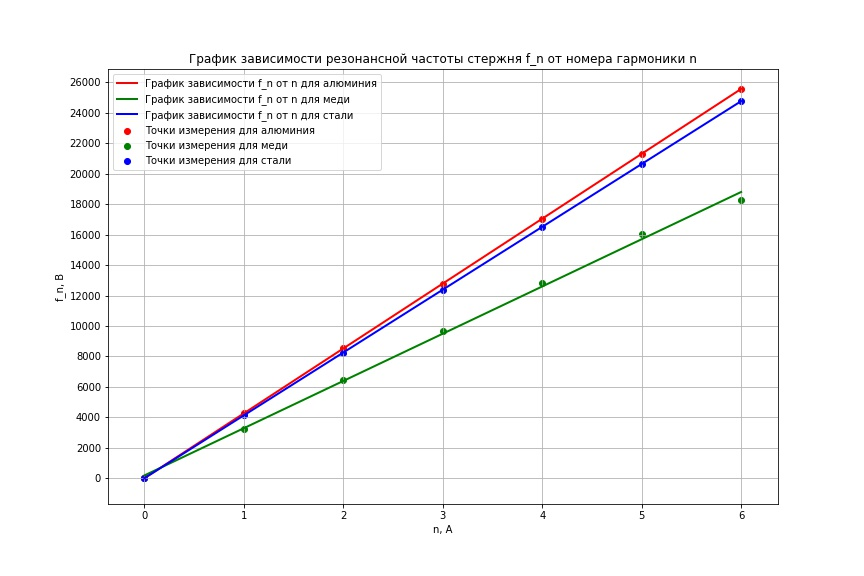
\includegraphics[width=15cm, height=11cm]{graph.jpg}
\end{center}

\begin{flushright}
{\scriptsize \textbf{Рис. 1.} \textbf {График зависимости частоты f от номера гармоники n.}}
\end{flushright}


    По полученным данным найдем значение скорости распространия волны $u$ из формулы \eqref{ф от н}.
    
    По методу наименьших квадратов для прямой, проходящей через начало координат найдем отношение $f_n/n$ для каждого из металлов:
    
    
\[k_{Al} = \frac{<xy>}{<x^2>} = 4264,2\]
\[\sigma_k = \sqrt{\frac{1}{n}\left(\frac{<y^2>}{<x^2>}-k^2\right)} = 0,4 (\varepsilon = 0,01\%)\]

\[k_{Cu} = 3146\]
\[\sigma_k = 34  (\varepsilon = 1,1\%)\]

\[k_{St} = 4128,5\]
\[\sigma_k = 0,7  (\varepsilon = 0,01\%)\]
    
    Погрешность полученной величины вычислим так:
    
\[\frac{\sigma_u}{u} = \sqrt{\left(\frac{\sigma_L}{L}\right)^2 + \left(\frac{\sigma_k}{k}\right)^2}\]



Для Алюминия:    
\[u = 5114,4 \pm 5,1 m/c^2\]
\[\varepsilon = 0,1\%\]

Для Меди:    
\[u = 3723,6 \pm 40,9 m/c^2\]
\[\varepsilon = 1,1\%\]

Для Стали:    
\[u = 4952,4 \pm 5,0 m/c^2\]
\[\varepsilon = 0,1\%\]




    Найдем модули Юнга для исследуемых материалов по формуле \eqref{скорость звука}:
    
    Погрешность результата будем вычислять по формуле:
    
\[\frac{\sigma_E}{E} = \sqrt{4\left(\frac{\sigma_u}{u}\right)^2 + \left(\frac{\sigma_{\rho}}{\rho}\right)^2}\]


    
Для Алюминия:    
\[E = u^2\rho = 73,9 \pm 0,4 GPa\]  \[\varepsilon = 0,6\%\]

Для Меди:    
\[E = u^2\rho = 127,2 \pm 2,8 GPa\]  \[\varepsilon = 2,2\%\]

Для Стали:    
\[E = u^2\rho = 189,2 \pm 0,6 GPa\]  \[\varepsilon = 0,3\%\]

(табл = 70 ГПа)
(табл = 110 ГПа)
(табл = 200 ГПа)




\section{Выводы}

    
    В ходе работы была экспериментально проверена линейность зависимости резонансной частоты стержня от номера гармоники гармонических колебаний. Для алюминия, меди и стали были получены модули Юнга этих металлов. Заметим, что основной вклад в погрешность итогового результата внесла погрешность нахождения плотности металлов. 
    
    Полученные значения отличаются от табличных более, чем на $3\sigma$. Это можно объяснить тем, что во время проведения эксперимента на итоговый результат оказывали сильное влияние непоперечные волны, из-за чего изображение на экране осциллографа было нечетким и полученные значения частот носят приближенный характер.

%\\\\\\\\\\\\\\\\\\\\\\\\\\\\\\\\\\\\\\\\\\\\\\\\\\\\\\\\\\\\\\\\\\\\\\\\\\\\\\\\\\\\\\\\\
%----------------------------------------------------------------------------------------------------------------

\end{document}
